\section{Diagramme}

\subsection{Domänenmodell}
Dieses Diagramm beschreibt das Problem (Die Umsetzung des Spiel), das gelöst werden muss.

\begin{figure}[htb]
 \begin{center}
  \leavevmode
  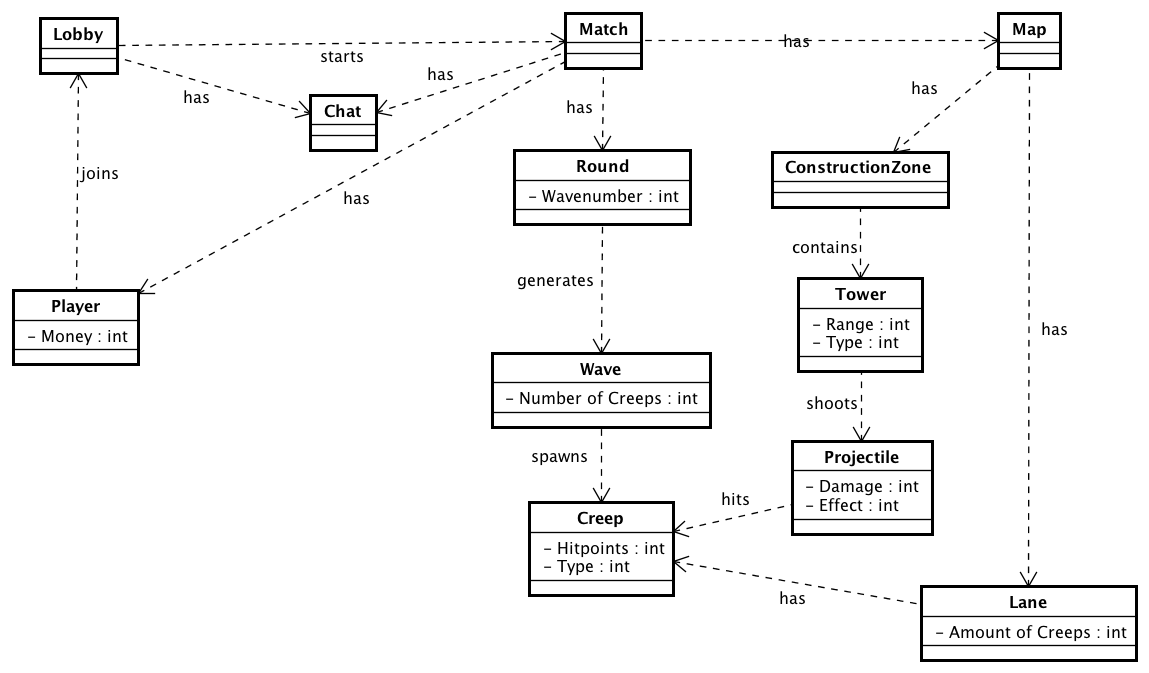
\includegraphics[width=1\textwidth]{domain_model.png}
 \end{center}
 \caption{Dom"anenmodell}
 \label{fig:Dom"anenmodell}
\end{figure}

\textbf{Erklährung des Diagrammes}

\textbf{Spieler}
\begin{itemize}
\item Diese Domäne beschreibt den Spieler, der am Spiel teilnimmt.
\end{itemize}

\textbf{Lobby}
\begin{itemize}
\item Im Multiplayerfall betreten die Spieler die Lobby, wo sie warten bis die gewünschte Anzahl Spieler erreicht ist. 
\end{itemize}

\textbf{Chat}
\begin{itemize}
\item Der Chat ermöglicht es den Spielern in der Lobby, wie auch im Spiel miteinander zu kommunizieren.
\end{itemize}

\textbf{Match}
\begin{itemize}
\item Organisiert das Spiel.
\item Beinhaltet die Map und kümmert sich um die einzelnen Runden.
\end{itemize}

\textbf{Round}
\begin{itemize}
\item Generiert die einzelnen Waves anhand der Anzahl Spieler.
\item Beinhaltet die Map und die \glossary{name={Lane}, description={Weg, auf welchem sich die Creeps bewegen}}{Lane}. Weiss in welchen Runde sich das Spiel befindet.
\end{itemize}

\textbf{Wave}
\begin{itemize}
\item Erzeugt die einzelnen Creeps, die zur Waves gehören.
\item Hat Informationen über Anzahl und Typ von Creeps die ge\glossary{name={to spawn}, description={erzeugen, generieren von creeps}}{spawn}t werden.
\end{itemize}

\textbf{Creep}
\begin{itemize}
\item Gegner, der sich auf dem Spielfeld befindet.
\item Hat Attribute wie Lebenspunkte und Typ.
\end{itemize}

\textbf{Map}
\begin{itemize}
\item Ist das eigentliche Spielfeld.
\item Beinhaltet die Constructionzone, sowie auch die Lane.
\end{itemize}

\textbf{Lane}
\begin{itemize}
\item Der Weg auf welchem sich die Creeps bewegen.
\item Kennt die Anzahl der Creeps, die sich momentan auf der Lane befinden.
\end{itemize}

\textbf{Constructionzone}
\begin{itemize}
\item Fläche auf der die Spieler Türme bauen können.
\end{itemize}

\textbf{Tower}
\begin{itemize}
\item Turm welcher auf der Constructionzone platziert werden kann.
\item Schiesst auf die Creeps
\end{itemize}

\textbf{Projectile}
\begin{itemize}
\item Projektil, welches von den Türmen geschossen wird.
\item Haben verschiedene Eigenschaften wie Schaden oder Effekte auf Creeps.
\end{itemize}

\newpage
\subsection{System-Sequenzdiagramm}
Dieses Sequenzdiagramm beschreibt die Systemoperationen des Use Cases UC1 ''Start Game''. Dabei wird ersichtlich, welche interaktionen der Benutzer in der Startphase des Programms tätigen kann und was dies bewirkt.

\begin{figure}[htb]
 \begin{center}
  \leavevmode
  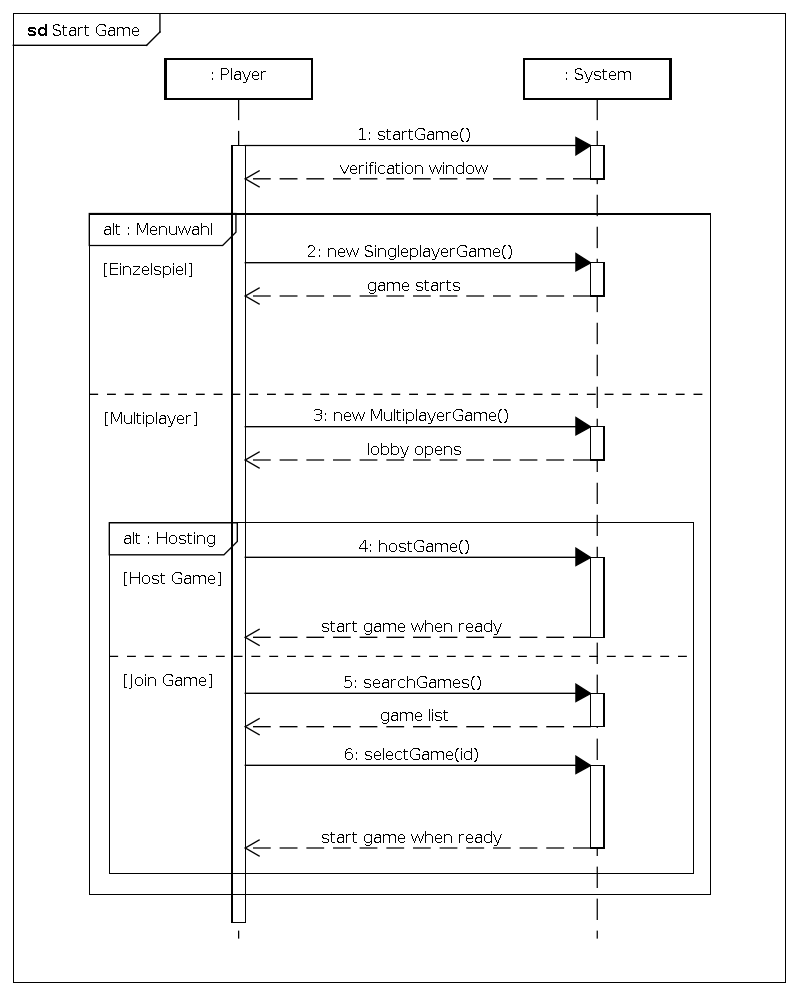
\includegraphics[width=0.85\textwidth]{SequenceDiagram.png}
 \end{center}
 \caption{Use Case UC1 ``Start Game'': Sequenzdiagramm}
 \label{fig:Sequenzdiagramm}
\end{figure}

%\subsection{Klassendiagramm}  (Müssen wir noch nicht machen)
